\documentclass[12pt,a4paper,twoside,openright,titlepage,final]{article}
\usepackage{fontspec}
\usepackage{amsmath}
\usepackage{amsfonts}
\usepackage{amssymb}
\usepackage{makeidx}
\usepackage{graphicx}
\usepackage[hidelinks,unicode=true]{hyperref}
\usepackage[spanish,es-nodecimaldot,es-lcroman,es-tabla,es-noshorthands]{babel}
\usepackage[left=3cm,right=2cm, bottom=4cm]{geometry}
\usepackage{natbib}
\usepackage{microtype}
\usepackage{ifdraft}
\usepackage{verbatim}
\usepackage[nottoc]{tocbibind}
\usepackage{pdflscape}
\usepackage{fancyvrb}
\usepackage[obeyDraft]{todonotes}
\ifdraft{
	\usepackage{draftwatermark}
	\SetWatermarkText{BORRADOR}
	\SetWatermarkScale{0.7}
	\SetWatermarkColor{red}
}{}
\usepackage{booktabs}
\usepackage{longtable}
\usepackage{calc}
\usepackage{array}
\usepackage{caption}
\usepackage{subfigure}
\usepackage{footnote}
\usepackage{url}
\usepackage[titletoc]{appendix}

\setsansfont[Ligatures=TeX]{texgyreadventor}
\setmainfont[Ligatures=TeX]{texgyrepagella}
\setmonofont{FreeMono}

\usetikzlibrary{decorations.pathreplacing}

%*******************************************************
%                 NO MODIFICAR
\newcommand*{\FSfont}[1]{%
  \fontencoding{T1}\fontfamily{#1}\selectfont}

\newlength{\tpheight}\setlength{\tpheight}{0.9\textheight}
\newlength{\txtheight}\setlength{\txtheight}{0.9\tpheight}
\newlength{\tpwidth}\setlength{\tpwidth}{0.9\textwidth}
\newlength{\txtwidth}\setlength{\txtwidth}{0.9\tpwidth}
\newlength{\drop}
%*******************************************************

% Crea una portada con los siguientes parámetros
%
% #1 : Título 
% #2 : Subtítulo
% #3 : Subsubtítulo
% #4 : Autor(es)
% #5 : Lugar
%

\newcommand*{\portada}[5]{
\begin{titlepage}
\begingroup
\vspace*{1cm}
\drop = 0.2\txtheight
\centering
\vfill
{\Huge \scshape #1}\\[\baselineskip]
{\Large \textbf{#2}}\\[\baselineskip]
{\Large \scshape #3}\\[\baselineskip]
\vspace*{0.3cm}
{\large \textit{#4}}\\[0.5\drop]

\includegraphics[scale=0.35]{./imagenes/logoURJC.jpg}
\vspace*{1.5cm}

{\large \scshape #5, \today} \par
\begin{center}
\end{center}
\vfill\null
\endgroup
\end{titlepage}
}
 %*****************************************************
 


\author{José Ignacio Escribano}

\title{}

\setlength{\parindent}{0pt}

\begin{document}

\pagenumbering{alph}
\setcounter{page}{1}

\portada{Foro de preguntas}{Análisis de Big Data}{Arquitecturas lambda y kappa}{José Ignacio Escribano}{Móstoles}

\tableofcontents
\thispagestyle{empty}
\newpage

\pagenumbering{arabic}
\setcounter{page}{1}

\section{Artículo}
\url{http://www.ericsson.com/research-blog/data-knowledge/data-processing-architectures-lambda-and-kappas}

¿Qué constituye una buena arquitectura para el procesado en tiempo real, cómo seleccionar la arquitectura correcta para un proyecto? En dos post, discutiremos las calidades de las dos arquitecturas más populares: la lambda y la kappa, y presentaremos ejemplos concretos de casos de uso implementando las distintas aproximaciones.\\

En este primer post, describimos las dos arquitecturas en más detalle: sus diferencias, las tecnologías que podemos utilizar para realizarlas así como los puntos claves que pueden decantarnos por una u otra.\\

Durante los últimos años, ha habido muchas discusiones sobre cómo diseñar una buena arquitectura en tiempo real. Una buena arquitectura en tiempo real necesita ser tolerante a fallos y escalable; necesita soportar batch y actualizaciones incrementales, y debe ser extensible.\\

Un importante hito en estas discusiones fue Nathan Marz, creador de Apache Storm, que nos daba a conocer la arquitectura lambda. La arquitectura lambda se ha probado que es relevante en muchos casos de uso y es, de hecho, usado por muchas compañías, como por ejemplo Yahoo y Netflix. Per, por supuesto, la arquitectura lambda no es solución mágica y ha recibido algunas críticas por la sobrecarga de código que puede crear.\\

En el verano de 2014, Jay Kreps, de LinkedIn, hizo un post describiendo lo que él llamaba la arquitectura kappa, que arreglaba alguna de los problemas que presentaba la arquitectura lambda. La arquitectura kappa no es un reemplazo de la arquitectura lambda, aunque, en algunos casos de uso desplegar con la arquitectura lambda no puede ser migrada.\\

Puede ser difícil evaluar con precisión qué arquitectura es la mejor para un caso de uso dado y tomar una decisión incorrecta de diseño puede tener grandes consecuencias para la implementación del proyecto de análisis de datos.\\

Ahora entraremos en más detalles de las dos arquitecturas de procesado de datos.\\

\begin{figure}[tbph!]
\centering
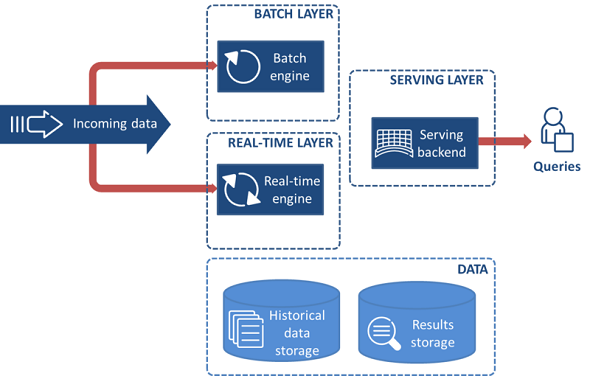
\includegraphics[width=0.7\linewidth]{imagenes/Lambda}
\caption{Arquitectura lambda}
\label{fig:Lambda}
\end{figure}

La arquitectura lambda, mostrada en la Figura~\ref{fig:Lambda}, se compone de tres capas: batch, de velocidad y de servicio.\\

La capa batch tiene dos tareas importantes: (a) manejar datos históricos; y (b) recalcular resultados como modelos de machine learning. Específicamente, la capa batch recibe datos entrantes, los combina con los datos históricos y recalcula los resultados iterando sobre el conjunto de datos entero. La capa batch opera sobre los datos completos y esto permite al sistema producir resultados más precisos. Sin embargo, los resultados tienen un coste alto que es la alta latencia, debida al gran tiempo de cálculo requerido.\\

La capa de velocidad es usada para proveer resultados con baja latencia, cercana al tiempo real. La capa de velocidad recibe los datos entrantes y devuelve actualizaciones incrementales a la capa batch. Gracias a los algoritmos incrementales, implementados en la capa de velocidad, el coste de cálculo es significativamente menor.\\

Finalmente, la capa de servicio habilita consultas de los resultados enviados desde las capa batch y de velocidad.\\

\begin{figure}[tbph!]
	\centering
	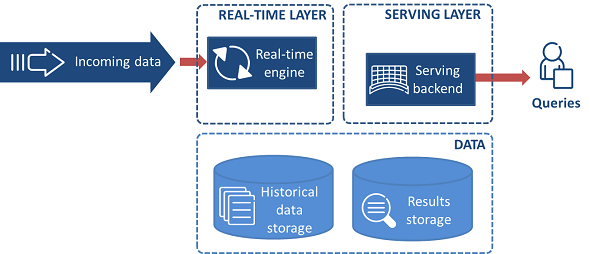
\includegraphics[width=0.7\linewidth]{imagenes/Kappa}
	\caption{Arquitectura kappa}
	\label{fig:Kappa}
\end{figure}  

La arquitectura kappa se muestra en la Figura~\ref{fig:Kappa}. Una de las motivaciones más importantes para inventar la arquitectura kappa es evitar mantener dos códigos para las capas de batch y velocidad. La idea clave es manejar ambas (procesado en tiempo real y el reprocesado de los datos continuos) usando un solo motor de procesado de streams. El reprocesado de datos en un importante requisito para hacer visible los efectos de los cambios de código en los resultados. Como consecuencias, la arquitectura kappa está compuesta de dos capas: copa procesamiento de stream y capa de servicio. La capa de procesamiento de stream corre los procesos de procesamiento de streams. El reprocesado de los datos sólo se hace cuando algo del código del proceso de procesamiento de stream debe ser modificado. Esto se logra corriendo otro proceso de procesamiento de stream modificado y replicando todos los datos anteriores. Finalmente, como en la arquitectura lambda, la capa de servicio se usa para consultar los resultados.\\

Las dos arquitecturas pueden ser implementadas combinando varias tecnologías open-source como Apache Kafka, Apache HBase, Apache Hadoop (HDFS, MapReduce), Apache Spark, Apache Drill, Spark Streaming, Apache Storm y Apache Samza.\\

Por ejemplo, los datos pueden ser ingeridos en las arquitecturas lambda y kappa usando un sistema de mensajería publicación-suscripción, como por ejemplo, Apache Kafka. El almacenamiento y modelado de datos puede ser implementado usando almacenamiento persistente como HDFS. Un sistema batch con alta latencia como Hadoop MapReduce puede ser usado en la capa batch de la arquitectura lambda para entrenar modelos desde cero. Sistemas de baja latencia como Apache Storm, Apache Samza y Spark Streaming puede ser usado para implementar modelos incrementales con actualizaciones del modelo en la capa de velocidad. Las misma tecnologías pueden ser usadas para implementar la capa de procesado de stream en la arquitectura lambda.\\

Alternativamente, Apache Spark puede ser usado como una plataforma común para desarrollar las capas batch y de velocidad en la arquitectura lambda. De esta manera, la mayoría del código puede ser compartido entre las capas de velocidad y batch. La capa de servicio puede ser implementada usando una base de datos NoSQL, como Apache HBase, y una motor de consultas SQL como Apache Drill.\\

Así que, ¿cuándo deberíamos usar una arquitectura u otra? Como en la mayoría de los casos, depende de la aplicación que estemos desarrollando. Veamos algunos ejemplos.\\

Un caso muy simple es considerar cuando los algoritmos aplicados a datos en tiempo real y datos históricos son idénticos. Es claramente beneficioso  usar el mismo código base para procesar los datos históricos y en tiempo real, y por tanto, implementar este caso de uso usando una arquitectura kappa.\\

Ahora, si los algoritmos para procesar los datos históricos y en tiempo real no son siempre idénticos. En algunos casos, el algoritmo batch puede ser optimizado gracias al hecho de que tenemos acceso al conjunto de datos histórico, y entonces mejorar la implementación del algoritmo en tiempo real. Aquí, elegir entre la arquitectura lambda y kappa se convierte a una elección entre el rendimiento favorable batch de ejecución sobre la simplicidad del código.\\

Finalmente, existen casos de uso más complejos, donde incluso las salidas los algoritmos batch y de tiempo real son diferentes. Por ejemplo, una aplicación de machine learning donde la generación del modelo batch requiere tanto tiempo y recursos que el mejor resultado en tiempo real es calcular y aproximar actualizaciones del modelo. En algunos casos, la capa batch y de tiempo real no pueden ser combinadas, y la arquitectura lambda debe ser usada.

\section{Preguntas}
\subsection{¿Cuáles son las principales diferencias entre el modelo de arquitectura lambda y arquitectura kappa para procesamiento de datos?}

La primera diferencia que se ve a simple vista es el número de capas de las que consta cada arquitectura. En la arquitectura lambda se tienen tres capas: batch, speed y serving, mientras que en la arquitectura kappa sólo se tienen dos capas: real-time y serving.\\

En la arquitectura lambda, la capa batch es la encargada de manejar datos históricos y recalcular resultados. Esto tiene una gran latencia debido a la gran cantidad de datos históricos, pero se consiguen mejores modelos, debido este elevado número de datos. La capa speed se usa para proveer datos resultados con baja latencia, llegando a estar cerca del real-time. Estos resultados se devuelven a la capa batch. Por último, la capa serving es la encargada de permitir realizar consultas enviadas desde las dos capas anteriores.\\

En la arquitectura kappa, se elimina la capa batch y se integra con la capa de speed en una nueva capa llamada real-time. Esta capa se encarga de procesar datos en tiempo real y sólo se reprocesan los datos cuando se ha modificado el código del proceso que realiza esta tarea. La capa serving se comporta de igual forma que en la arquitectura lambda.\\

Debido a esta diferencia en el número de capas, la arquitectura lambda debe mantener código duplicado en las capas batch y speed. Ésta es una de las razones de la invención de la arquitectura kappa, ya que evita la duplicidad de código combinando la capa batch y speed en una única capa.  

\subsection{¿Cuáles son las principales ventajas de usar Apache Spark en la implementación de una arquitectura lambda?}

De acuerdo al artículo, el uso de Apache Spark en la implementación de una arquitectura lambda, permite desarrollar las capas batch y speed de manera que la mayoría del código sea compartido por ambas capas, pudiendo reducir el tiempo de implementación de la aplicación con esta arquitectura, y minimizando el tiempo de mantenimiento del código de ambas capas.

\end{document} 